\usetikzlibrary{decorations.markings}


\tikzset{test/.style n args={3}{
			postaction={
					decorate,
					decoration={
							markings,
							mark=between positions 0 and \pgfdecoratedpathlength step 0.25pt with {
									\pgfmathsetmacro\myval{multiply(
										divide(
										\pgfkeysvalueof{/pgf/decoration/mark info/distance from start}, \pgfdecoratedpathlength
										),
										100
										)};
									\pgfsetfillcolor{#3!\myval!#2};
									\pgfpathcircle{\pgfpointorigin}{#1};
									\pgfusepath{fill};}
						}}}}

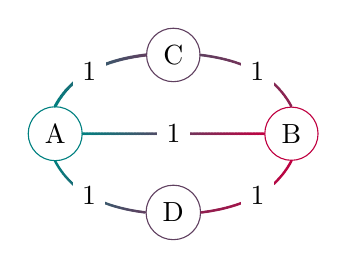
\begin{tikzpicture}[yscale=.5, xscale=.75]
	\node[draw=teal, circle] (A) at (0, 0) {A};
	\node[draw=purple, circle] (B) at (4, 0) {B};
	\node[draw=teal!50!purple, circle] (C) at (2, 2) {C};
	\node[draw=teal!50!purple, circle] (D) at (2, -2) {D};

	\draw[test={.6pt}{teal}{teal!50!purple}]
	(A.north) to[bend left] node[fill=white, rectangle, midway] {$1$} (C.west);
	\draw[test={.5pt}{teal}{teal!50!purple}]
	(A.south) to[bend right] node[fill=white, rectangle, midway] {$1$} (D.west)
	;
	\draw[test={.5pt}{teal}{purple}]
	(A.east) to node[fill=white, rectangle, midway] {$1$} (B.west);
	\draw[test={.5pt}{teal!50!purple}{purple}]
	(C.east) to[bend left] node[fill=white, rectangle, midway] {$1$} (B.north)
	(D.east) to[bend right] node[fill=white, rectangle, midway] {$1$} (B.south)
	;

\end{tikzpicture}
